\section{Durchführung}
\label{sec:durchführung}

Abbildung~\ref{fig:aufbau} zeigt schematisch den Aufbau der Messapparatur, sowie die verwendete Schaltung. An dem oben bereits beschriebenen Szintillator befinden sich an beiden Seiten die Sekundär-Elektronen-Verstärker. Diese wandeln die von den Photonen erzeugten Elektronen in digitale Spannungssignale um. Dazu werden sie mit Hochspannung versorgt. Die so erzeugten Signale werden über Verzögerungsleitungen von beiden Seiten des Szintillators an zwei Kanäle eines Diskriminators gelegt. Die Verzögerungsleitungen dienen dabei dem Ausgleich der Zeitspannen zwischen Erzeugung eines eines Photons und Ankunft des dazugehörigen digitalen Signals am Diskriminator. So lässt sich die Zahl der ermittelten Ereignisse maximieren. Der Diskriminator besitzt eine variable Schwelle, ab welcher Signale als solche gewertet werden. Dieses unterdrückt das natürliche Rauschen. Signale, die als solche gewertet werden, werden darüber hinaus in NIM Logik entsprechende Signale gleicher Amplitude gewandelt. Diese Signale erreichen anschließend die sogenannte Koinzidenz-Schaltung. Diese sorgt dafür, dass Impulse, die in einem gewissen Zeitintervall $\upD t$ die Schaltung erreichen als gleichzeitig gelten. Solche Impulse werden anschließend an die beiden AND-Gatter weitergeleitet. \\
Weil nur wenige Myonen zwei Lichtimpulse im Szintillator erzeugen, also so niederenergetisch sind, dass sie im Szintillator zerfallen, ist mit deutlich mehr "Start"- als "Stop"-Impulsen zu rechnen. Die im unteren Teil des Diagramms dargestellte Schaltung dient dem Zweck dennoch möglichst nur die physikalisch sinnvollen Zeitintervalle aufzunehmen. Dazu wird die "Wartezeit" bis zum Stop-Impuls begrenzt. Die Ausgangssignale der Koinzidenzschaltung gelangen an das erste AND-Gatter und aktivieren so den START-Eingang des TAC. Dieser \textit{time-amplitude-converter} sorgt dafür, dass die gemessenen Zeiträume digitalisiert und in verschiedenen Kanälen gespeichert werden. Außerdem wird eine so genannte Kippstufe angestoßen. Diese Kippstufe legt für eine begrenzte Zeit $T_s$ ein Signal an das zweite AND-Gatter. Zerfällt das Myon in diesem Zeitraum im Tank und sendet somit die Koinzidenzschaltung einen Stop-Impuls, so gelangt dieses zum STOP-Eingang des TAC und ein Messwert wird generiert. Nach Ablauf dieses Zeitraums beendet die Kippstufe ihr Signal und die Schaltung begibt sich wieder in den Anfangszustand. Signale die nach diesem Zeitraum eintreffen werden also wieder als Start-Impulse registriert. Die Länge des Zeitraumes sollte daher so gewählt werden, dass die tatsächliche Dauer von Start-Impuls und Zerfall eines Myons deutlich kleiner ist (damit alle realen Signale auchh eingefangen werden) allerdings kleiner als die erwartete Zeitspanne in welcher zwei zufällige Myonen in den Szintillator vordringen, sodass diese möglichst nicht als der Zerfall eines Myons interpretiert werden.
%
\begin{figure}[htb]
  \centering
  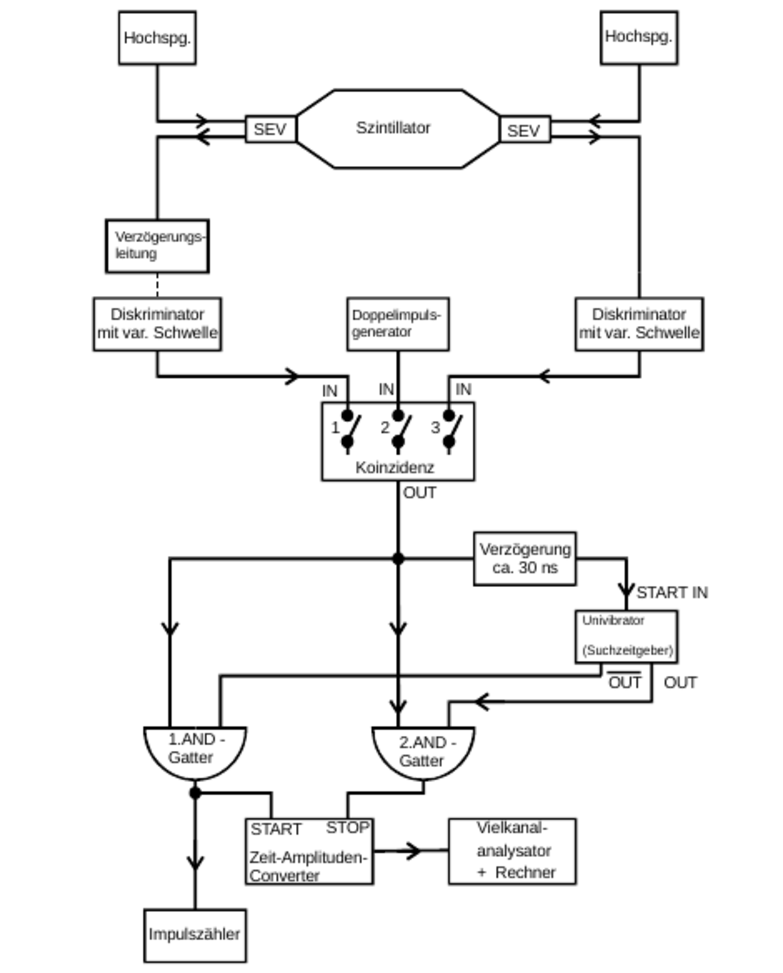
\includegraphics[width=0.6\textwidth]{figures/versuchsaufbau.pdf}
  \caption{Schematischer Aufbau der Versuchsapparatur und der damit verbundenen Schaltung. \cite{V01}}
  \label{fig:aufbau}
\end{figure}
%
\subsection{Durchführung}

Die Durchführung dieses Versuches gliedert sich in zwei Teile: zunächst wird die Schaltung aufgebaut und die einzelnen Komponenten getestet. Die Schaltung wird so eingestellt, dass die gemessene Rate maximal wird und anschließend eine Kalibrationsmessung durchgeführt. Ist die Messapparatur betriebsbereit, wird die Messung gestartet und im zweiten Teil die Daten aufgenommen. \\
Zur Einstellung der Messschaltung sind zunächst die Diskriminatoren einzustellen. Diese werden mit Hilfe von Impulsen und einem Oszilloskop so eingestellt, dass die Höhen und Breiten (also Dauern) der Impulse, die den Diskriminator verlassen einheitlich sind. Anschließend sind die zeitlichen Differenzen der Signale der verschiedenen SEV auszugleichen. Dazu werden diese über Verzögerungsleitungen relativ zueinander verzögert. Es wird eine feste Verzögerung für eine Leitung festgelegt und relativ dazu die Verzögerung der anderen variiert. Das Ziel ist hierbei eine möglichst hohe Zählrate zu generieren, ergo die Impulse möglichst übereinander zu legen. Dazu wird eine Messreihe der Zählrate in Abhängigkeit der relativen Verzögerung der beiden Kanäle zueinander durchgeführt. \\
Um die so eingestellte Apperatur zu überprüfen wird die Funktion der Koinzidenzschaltung überprüft. Die Zählrate sollte von dieser im Vergleich zu der nach den Diskriminatoren auftretenden noch deutlich reduziert werden. \\
Bevor nun die Messung gestartet werden kann, muss noch die Kalibrierung der Zeitkanäle des TAC vorgenommen werden. Dazu werden von einem Doppelimpulsgenerator Impulse verschiedener zeitlicher Abstände an den TAC geleitet und anschließend am Rechner gespeichert. Durch Vermessen verschiedener Zeitintervalle lassen sich den 511 Kanälen die zugehörigen Zeitintervalle zuordnen. \\
Nach dieser Kalibrierung kann die Messung gestartet werden. Die Schaltung darf dabei nach der Kalibrierung nicht mehr verändert werden. Am Rechner wird das Messprogramm gestartet und über eine Dauer von 20-30h Daten genommen.
